\documentclass[12pt]{article}

\usepackage{amsmath,amssymb}
\usepackage{graphicx}

\usepackage{setspace}
\onehalfspacing
\usepackage[margin=1in]{geometry}
\usepackage{hyperref}
\hypersetup{linkcolor=blue, allcolors=true}
\usepackage[utf8]{inputenc}
% Notation
% Mathematical functions
\newcommand{\isone}[1]{{\boldsymbol{1}\left( #1 \right)}}
\renewcommand{\Pr}[1]{{\mathbb{P}\left(#1\right) }}
\newcommand{\f}[1]{{f\left(#1\right) }}
\newcommand{\Prcond}[2]{{\mbox{Pr}\left(#1\vphantom{#2}\;\right|\left.\vphantom{#1}#2\right)}}
\newcommand{\fcond}[2]{{f\left(#1|#2\right) }}
\newcommand{\Expected}[1]{{\mathbb{E}\left\{#1\right\}}}
\newcommand{\ExpectedCond}[2]{{\mathbb{E}\left\{#1\vphantom{#2}\;\right|\left.\vphantom{#1}#2\right\}}}

\newcommand{\Likelihood}[2]{\text{L}\left(#1 \left|\vphantom{#1}#2\right.\right)}
\newcommand{\sufstats}[1]{s\left(#1\right)}
\renewcommand{\exp}[1]{\mbox{exp}\left\{#1\right\}}
\newcommand{\transpose}[1]{{#1}^\mathbf{t}}

% Objects
\newcommand{\params}{\theta}
\newcommand{\Params}{\Theta}
\newcommand{\Graph}{\mathbf{G}}
\newcommand{\graph}{\mathbf{g}}
\newcommand{\GRAPH}{\mathcal{G}}
\newcommand{\Adjmat}{Y}
\newcommand{\adjmat}{y}
\newcommand{\ADJMAT}{\mathcal{Y}}

\newcommand{\INDEPVAR}{\mathcal{X}}
\newcommand{\Indepvar}{X}
\newcommand{\indepvar}{x}

\newcommand{\normconst}{\kappa\left(\params, \Indepvar\right)}

% \graphicspath{{./fig/}}


%% NEED THIS FOR CANCY TEX
\usepackage{pstricks}

% Colors
\definecolor{USCCardinal}{HTML}{990000} % 153 0 0 in RGB
\definecolor{USCGold}{HTML}{FFCC00}
\definecolor{USCGray}{HTML}{CCCCCC}

% To use the function \sout
\usepackage{ulem}
\usepackage{tabularx, booktabs}

% \bibliography{bibliography.bib}

\title{Exponential Random Graph models for Little Networks}
\author{George G. Vega Yon \and Kayla de la Haye}
\date{January 2019}

\begin{document}

\maketitle

To be submitted at https://arxiv.org/help/submit

\section{Introduction}

\section{Exponential-Family Random Graph Models}

Exponential-Family Random Graph Models (ERGMs), are certainly one of the most popular tools used by social scientists interested on understanding social networks \cite[and others]{Robins2007,Holland1981,Wasserman1996,Snijders2006}. In this family of models, an observed graph $\adjmat$, or more commonly put, its adjacency matrix representation, is characterized by a set of sufficient statistics, which we denote $\sufstats{}$, as follows:

\begin{equation}
\label{eq:ergm}
  \Prcond{\Adjmat = \adjmat}{\params, \Indepvar} = \frac{%
  	\exp{\transpose{\params}\sufstats{\adjmat, \Indepvar}}%	
  }{
  	\kappa\left(\params, \Indepvar\right)
  },\quad\forall \adjmat\in\ADJMAT
\end{equation}

\noindent Where $\normconst{} = \sum_{\adjmat\in\ADJMAT}\exp{\transpose{\theta}\sufstats{\adjmat, \Indepvar}}$ is the normalizing constant, and $\ADJMAT$ is the support of the model which is usually assumed to include all directed graphs of the same size as $\adjmat$, that are directed, and do not include self-ties; in this particular case, the size of $\ADJMAT$ equals $2^{n(n-1)}$ possible graphs. Such makes the exact calculation of $\normconst{}$, and hence of \eqref{eq:ergm} extremely complicated to calculate.

\def\fig1width{.45\linewidth}
\begin{figure}
\centering
\begin{tabular}{m{.2\linewidth}<\centering m{.4\linewidth}<\raggedright}
\toprule Representation & Description  \\ \midrule

\includegraphics[width=\fig1width]{terms/mutual.pdf} & Mutual Ties (Reciprocity)\linebreak[4]$\sum_{i\neq j}y_{ij}y_{ji}$  \\
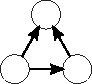
\includegraphics[width=\fig1width]{terms/ttriad.pdf} & Transitive Triad (Balance)\linebreak[4]$\sum_{i\neq j\neq k}y_{ij}y_{jk}y_{ik}$  \\

\includegraphics[width=\fig1width]{terms/homophily.pdf} & Homophily\linebreak[4]$\sum_{i\neq j}y_{ij}\mathbf{1}\left(x_i=x_j\right)$ \\
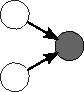
\includegraphics[width=\fig1width]{terms/nodeicov.pdf} & Covariate Effect for Incoming Ties\linebreak[4]$\sum_{i\neq j}y_{ij}x_j$ \\
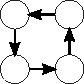
\includegraphics[width=\fig1width]{terms/fourcycle.pdf} & Four Cycle\linebreak[4]$\sum_{i\neq j \neq k \neq l}y_{ij}y_{jk}y_{kl}y_{li}$  \\
\bottomrule
\end{tabular}
\caption{\label{fig:ergm-structs}Besides of the common edge count statistic (number of ties in a graph), ERGMs allow measuring other more complex structures that can be captured as sufficient statistics. }
\end{figure}

Ultimately, while mentioned several times throughout the literature \cite{Wasserman1996,Frank1986,Snijders2011}, the use of exponential random graph models for "small networks" (which we will describe as those networks in which enumerating the entire support of the distribution is possible using modern computers) is not observed as often as in the case of "larger" networks, leave alone calculating the likelihood function using exhaustive enumeration (which we will refer as exact likelihood) instead of simulation-based estimation methods as done today in the most popular software packages used for estimating these models. One key aspect of this is the fact that simulation-based estimation methods have not been developed with this in mind.\footnote{Perhaps because that, as put by \cite{Snijders2011}, small networks are considered to be "uninteresting special cases"}

The infamous degeneracy problem \cite{Handcock2003} that users of this method encounter too often is more prevalent in the case of small networks. For example, if we are trying to estimate an ERGM in a network with only two nodes, in the scenario where such graph is directed and does not allow for self-ties, the chances of obtaining either a fully connected or a fully empty graph are exactly half. The problem, while less prevalent, is still observed more often compare to what we would see in in networks with more nodes, say 8 for example, and it hardly goes away as the sample size increases. In fact, the degeneracy problem has such high prevalence in small networks that most practitioners find it futile.\footnote{In some cases, researchers try to aggregate their data, if using multiple networks, such that to be able to obtain something similar to pooled estimates. In order to do so, practitioners stack multiple adjancency matrices as a single one building a block-diagonal dataset, explicitly modeling the networks as independent by fixing the "off diagonal" components to zero (structural zeros). The problem with this approach lies on the fact that the very set of constraints that are subscribed to the model make the sampling procedure complicated.} The good news, the degeneracy problem is not present in the cases in which likelihood function is trackable. In this paper, we present a revisit of the Exponential Random Graph Models for small networks, the estimation process that can be used in such case, and some results from an extensive simulation study that we conducted.

\section{ERGM{\it{}itos}: ERGMs for small networks}

In modern computers, calculating the exact likelihood function of an exponential random graph model for a small network becomes computationally feasible. This has an important implication: the estimation process of the parameters of an ERGMs of a small networks can be done directly without having to use simulations like modern methods do when fitting this kind of models. This way, besides of obtaining a better solution (in general), if the MLEs exists, we avoid the degeneracy problem. It is important to notice that, while the degeneracy problem is not completely avoided, we are indeed reaching a better situation compared to what we would get if we were using MC-MLE estimation, for example. One result by \cite[p. 7]{Handcock2003}, "[i]f the model used to simulate the graphs is not close enough to produce realizations that cover the observed values of the statistics, the MC-MLE will not exist even in cases where the MLE does.", in other words, while the non-existence of MLE estimates implies the non-existence of MC-MLE estimates, the opposite is not true.

Since most of small network data comes in the form of multiple networks--for example, families, small teams, ego-networks, etc.--assuming that the data generating process is shared across the sampled networks, then obtaining pooled estimates is a natural way of estimating of modeling the graphs. Pairing up the previous assumption with an independence independence across graphs, allows us calculating the exact likelihood function for pooled estimates by maximizing the following:

\begin{equation}
    \label{eq:ergm-pooled}
    \Prcond{\Adjmat_1 = \adjmat_1, \dots, \Adjmat_P = \adjmat_P}{\params, \Indepvar_1, \dots, \Indepvar_p} = \prod_{p=1}^P\frac{%
    		\exp{\transpose{\params}\sufstats{\adjmat_p, \Indepvar_p}}%	
    	}{
    		\kappa_p\left(\params, \Indepvar_p\right)
    	}
\end{equation}

\noindent Where $P$ denotes the number of networks used in the model. We call this model ERGMito\footnote{The \textit{ito}/\textit{ita} suffix is used in Spanish to denote small, or affection. We are particularly grateful to George Barnett who proposed the name during the North American Social Networks Conference on 2018.}.

One potential problem that we are not addressing with the pooled estimates is the problem of scalability, in particular, the interpretation of the constant parameter in the model, the edge count parameter. In the baseline case of estimating a density parameters using a single network, as pointed out in \cite{Krivitsky2011}, extrapolating or comparing those estimates in the context of a network with a different size may be a bit complicated in the sense that, if left as is, a fixed density parameter assumes a constant change in the average degree of the network, which may not be realistic in some scenarios, as instead it may be more natural to think that the degree holds constant. Still, the cases pointed out by \cite{Krivitsky2011} discuss situations in which the sizes of the networks range from a few dozens to a couple of thousands, which will not be the case here.

The simulations and model fitting were conducted using the R package \texttt{ergmito} which has been developed to implement the methods described in this work.

\section{Illustration with simulated data: fivenets}

In what follows we will work with a toy dataset generated using the data-generating-process of ERGMitos. This particular dataset, which we call ``fivenets'', is included in the in the R package \texttt{ergmito}. The dataset contains five simulated networks, each using the following model:

\begin{multline*}
\Prcond{\Adjmat = \adjmat}{\Indepvar_{\mbox{gender}}, \params} = \\
\frac{ %
    \exp{\params_{edges}\left(\sum_{i,j} \adjmat_{ij}\right) + %
    \params_{homophily}\left(\sum_{i,j} \adjmat_{i}\isone{\Indepvar_{gender, i} = \Indepvar_{gender, j}}}\right) %
    }{%
    \normconst{}
    }
\end{multline*}

Using the previous equation, we draw five networks of size five. In the case of the ``homophily'', parameter which is operationalized as the number of ties in which ego and alter have the same gender, before drawing the networks, we randomly generated the gender parameter to each vertex as a Bernoulli with parameter 0.5. \autoref{fig:fivenets} shows the five networks.

\begin{figure}
    \centering
    \includegraphics{}
    \caption{\label{fig:fivenets}Caption}
    \label{fig:my_label}
\end{figure}


\autoref{fivenets:coefficients} shows the estimation results of three different especifications of the model: (1) Homophily only, (2) Edgecount only, and (3) Full model (both parameters).

\begin{table}
\begin{center}
\begin{tabular}{l c c c }
\hline
 & Homophily only & Edgecount only & Full model \\
\hline
nodematch.female & $-0.12$  &             & $1.59^{*}$   \\
                 & $(0.34)$ &             & $(0.64)$     \\
edges            &          & $-0.69^{*}$ & $-1.70^{**}$ \\
                 &          & $(0.27)$    & $(0.54)$     \\
\hline
AIC              & 85.06    & 78.38       & 73.34        \\
BIC              & 87.15    & 80.48       & 77.53        \\
Log Likelihood   & -41.53   & -38.19      & -34.67       \\
Num. networks    & 5        & 5           & 5            \\
\hline
\multicolumn{4}{l}{\scriptsize{$^{***}p<0.001$, $^{**}p<0.01$, $^*p<0.05$}}
\end{tabular}
\caption{Fitted ERGMitos using the fivenets dataset. As expected, the Full model (last column of the table) has overall a better fit of the data (higher LogLikelihood value), more over, the observed coefficients for both statistics are inline with the true parameters.}
\label{fivenets:coefficients}
\end{center}
\end{table}

Practitioners of ERGMs should be familiar with the goodness-of-fit diagnostic performed every time a model is fitted. In general, the most looked statistics are the distribution of shortest-path lengths, and .... In the case of ERGMitos, such parameter loses some relevance since, in general, the shortest-path lengths between any two nodes lies usually (or at least there is a high chance of) between 1 and 2 steps. \autoref{fig:fivenets-gof} shows the GOF statistics for the model parameters.

An important advantage of the ERGMitos over ``regular'' ERGMs is that we can observe the surface of the log-likelihood over different combination of parameters in a rather straightforward way. This, together with the goodness-of-fit analysis should be a routine thing to be done after every ERGMito fit. \autoref{fig:fivenets-loglike} shows the surface of the log-likelihood function around the solution.

\begin{figure}
    \centering
    \caption{Goodness-of-fit in ERGMitos. In this case we are showing how do the observed sufficient statistics of each one of the 5 networks (x-axis) locate in the overall estimated distribution based on the fitted ERGMito. The gray lines in each box show the minimum and maximum value that the sufficient statistics can take in each one of the 5 networks, whereas the dotted lines provide a 90\% confidence interval. The dots are the observed statistics in each network.}
    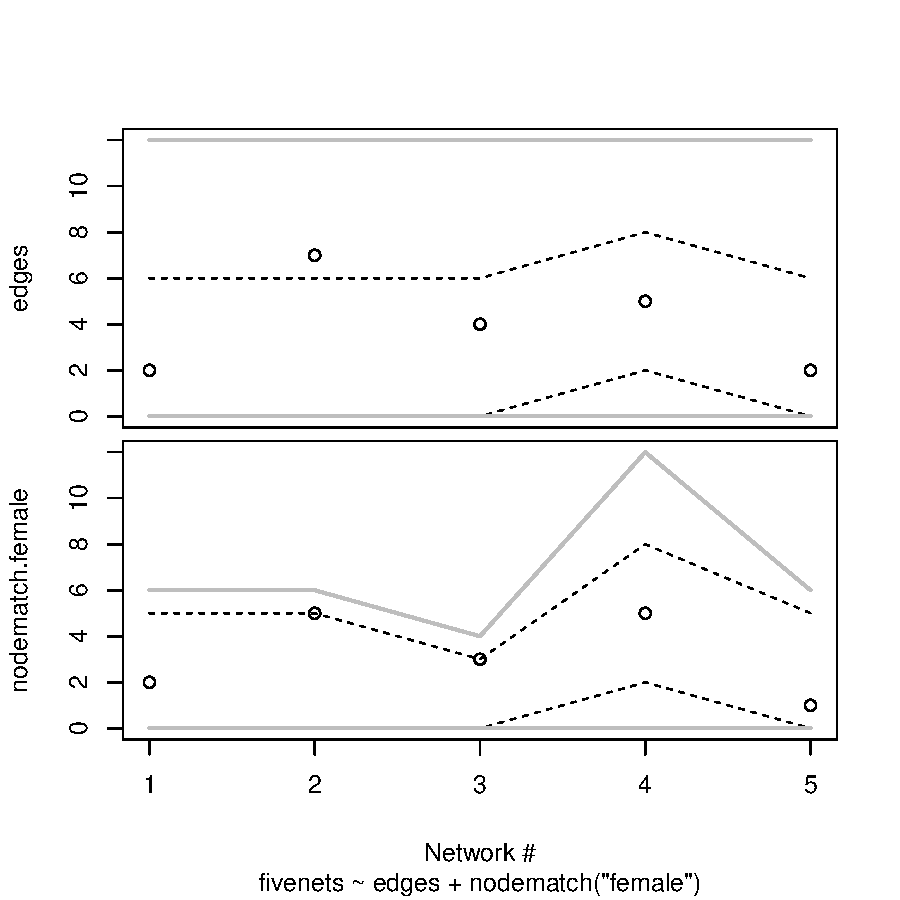
\includegraphics[width=.7\linewidth]{figures/fivenets_gof.pdf}
    \label{fig:fivenets-gof}
\end{figure}

\begin{figure}
    \centering
    \caption{Surface of the log-likelihood function of the pooled ERGMito model. Lighter colors represent higher values while darker ones represent lower values. The red dot corresponds to the location of the MLE estimate of the model.}
    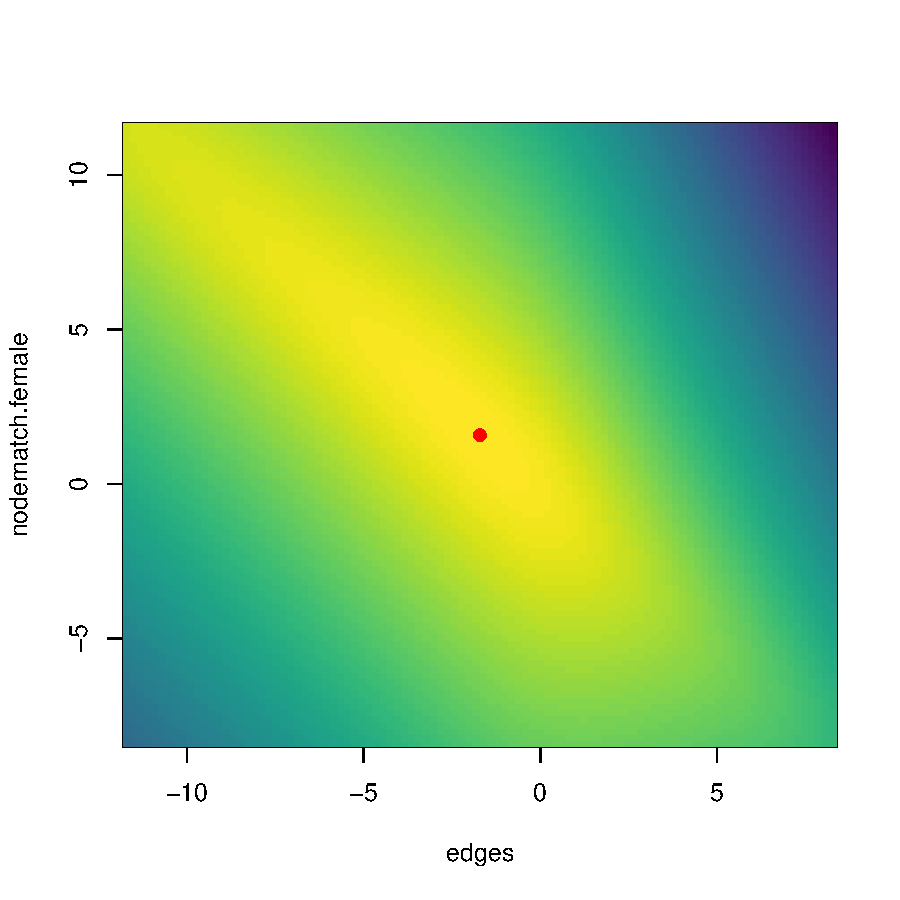
\includegraphics[width=.7\linewidth]{figures/fivenets_loglike.pdf}
    \label{fig:fivenets-loglike}
\end{figure}

\section{Simulation study}

We conducted a simulation study to explore the properties of MLE for small networks. To generate each sample of teams:

1. Draw the **population parameters** from a piece-wise Uniform with values in $[-4, -.1]\cup[.1, 4]$

2. We will draw groups of sizes 3 to 5. The number of networks per group size are drawn from a Poisson distribution with parameter 10 (hence, an expected size of 30 networks per sample).

3. Use the drawn parameters and group sizes to generate random graphs using an ERGM data generating process.

We simulated 100,000 samples, each one composed of an average of 30 networks.

\begin{figure}
	\centering
	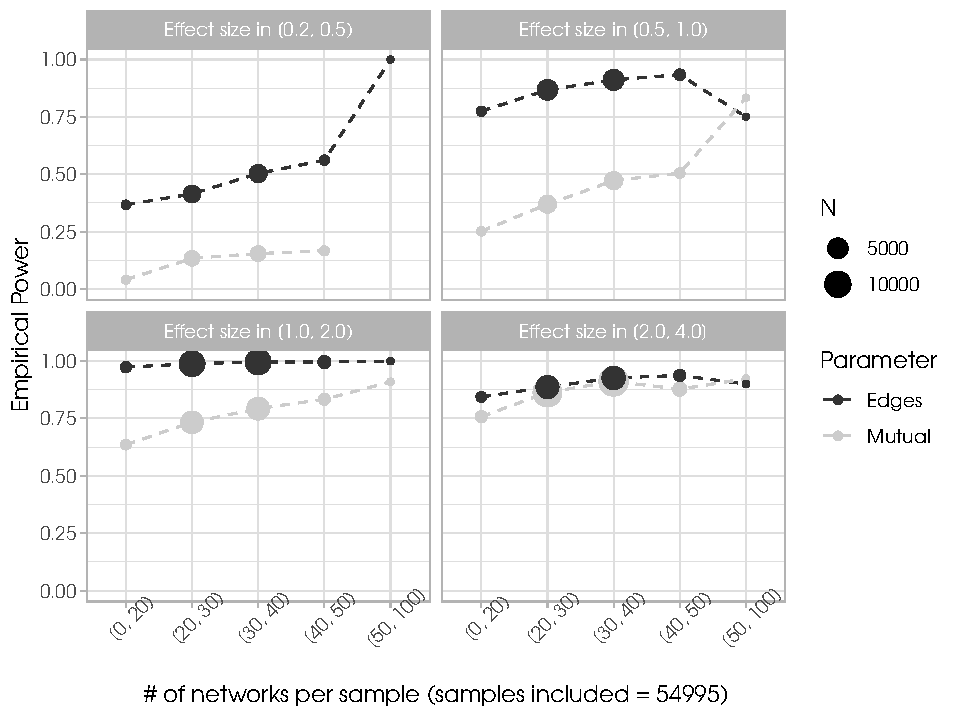
\includegraphics[width=.9\linewidth]{power-02-various-sizes-3-5.pdf}
\end{figure}

\section{Discussion}

\section{Acknowledgements}

This material is based upon work support by, or in part by, the U.S. Army Research Laboratory and the U.S. Army Research Office under grant number W911NF-15-1-0577

Computation for the work described in this paper was supported by the University of Southern California’s Center for High-Performance Computing (hpcc.usc.edu).

\bibliographystyle{plain}
\bibliography{bibliography.bib}

\appendix

\section{MLE}

In order to improve accuracy of the estimation process, we use both the log-likelihood function and its gradient to find the MLEs. In particular, in this iteration of the manuscript we are using the BFGS quasi-newtonian optimization algorithm as provided by the R package stats in the optim function. In the general case, whether we have one or more networks (pooled estimates), the gradient of the log-likelihood function can be calculated as follows:

\begin{equation}
\sum_{p}\nabla l_p(\theta) = \transpose{\sufstats{\adjmat_p, \Indepvar_p}} - \frac{\transpose{Q_p}\left(\transpose{W_p} \circ \exp{Q_p \theta}\right)}{\kappa_p}
\end{equation}

Where $\sufstats{\adjmat, \Indepvar}$ is a vector of observed sufficient statistics (usually called target statistics), $Q$ is a matrix of sufficient statistics, in particular, the isomorphic sufficient statistics associated with the model, and $W$ is a vector of frequency weights.


\end{document}
